% ICMLDE 2026 submission
% Based on the Procedia Computer Science CRC template (Elsevier ecrc.sty)
\documentclass[3p,times,procedia]{elsarticle}
\flushbottom

\usepackage{ecrc}
\usepackage[bookmarks=false]{hyperref}
    \hypersetup{colorlinks,
      linkcolor=blue,
      citecolor=blue,
      urlcolor=blue}
\usepackage{amssymb}
\usepackage{graphicx}
\usepackage{booktabs}

\volume{00}
\firstpage{1}
\journalname{Procedia Computer Science}
\runauth{Kavinesh P et al.}
\jid{procs}

\begin{document}
\begin{frontmatter}

\dochead{International Conference on Machine Learning and Data Engineering}

\title{Why AI-Generated Image Detectors Fail on Modern Diffusion Generators: A Cross-Architecture Generalization and Failure-Mode Analysis}

\author[a]{Kavinesh P}
\author[a]{Raam Prathap R V}
\author[a]{Santhosh A S}
\author[a]{Kasam Sai Venkata Siddardha}
\author[a]{Ashish M}
\author[a]{M Anbazhagan\corref{cor1}}

\address[a]{Department of Computer Science and Engineering, Amrita School of Computing, Coimbatore 641112, Amrita Vishwa Vidyapeetham, India}

\begin{abstract}
AI-generated image detectors are usually reported as a single accuracy
number against a fixed test set, which hides two questions that matter more
for deployment: does accuracy on one generator predict accuracy on another,
and when a detector fails, does it fail by being uncertain or by being
confidently wrong? We evaluate five pretrained, publicly released detectors
against five generators spanning three architecture families (GAN, early
and modern U-Net diffusion, and Diffusion Transformer), with every
generator verified absent from every detector's training data, at a fixed
0.5 threshold, reporting both classes and threshold-free AUC throughout.
This paper makes four contributions. First, a generalization audit showing
that detectors disagree about which generator is hard: one fails worst on
FLUX.1 (7.0\% fake-accuracy), another on SDXL (54.6\%), two others on
BigGAN (0.4\% and 9.6\%), and paired McNemar tests on identical image sets
confirm these gaps are significant, with one informative exception where
two same-lineage detectors are statistically indistinguishable
($p=0.098$). Second, a decomposition of that disagreement: two detectors
trained on identical data but with different architectures produce an
\emph{identical} difficulty ordering across all five generators
($\rho=+1.000$, exact $p=0.017$) while differing by 37.6 points in mean
accuracy, suggesting training data sets the shape of a detector's failure
profile and the representation sets its level. Third, a calibration
account of how detectors fail: expected calibration error rises with
failure severity rather than falling, reaching 0.503 where fake-accuracy is
0.4\%, so these models do not degrade into uncertainty as they leave their
training distribution, they stay confident and become wrong. Fourth, a
reproducibility finding: a resize convention that is rarely specified in
released code moves the same checkpoint's reported accuracy on the same
benchmark by more than 15 points, in opposite directions for two
checkpoints trained on identical data, which we trace, replicate on a
second generator, and decompose into a recoverable threshold shift and an
information-destroying input distortion. Adversarial training on
on-manifold latent perturbations (a published method we evaluate but did
not modify) raises mean fake-accuracy from 66.2\% to 98.7\% and yields the
best-calibrated detector we test. We also report two cautions that apply
beyond our own pipeline: the strongest detector on clean FLUX.1 data
(98.0\% fake-accuracy) drops to chance-level AUC under ordinary JPEG
re-encoding, and every generator in these benchmarks ships generated images
as PNG against JPEG reals, a compression confound that inflates absolute
accuracies. Everything is produced by inference over existing checkpoints
and released datasets, with no training and no image generation, so the
pipeline is reproducible on a single consumer GPU.
\end{abstract}

\begin{keyword}
AI-generated image detection \sep synthetic image forensics \sep cross-generator generalization \sep diffusion models \sep adversarial training \sep calibration \sep reproducibility
\end{keyword}
\cortext[cor1]{Corresponding author: M Anbazhagan}
\end{frontmatter}

\email{m\_anbazhagan@cb.amrita.edu}

\vspace*{-6pt}

\section{Introduction}
\label{sec:intro}

A detector's accuracy number is only useful if it predicts behavior on data
the detector has not seen. In practice, a detector trained on one
generator's outputs is regularly reported to lose most of its accuracy on a
different generator's outputs, and the field has largely explained this with
a single story: newer, more sophisticated generators produce artifacts that
older detectors were not built to catch. That story predicts a specific
pattern. Detectors should fail worst on the newest generators, and that
failure should look broadly similar across detectors that were not trained
on them.

We test the prediction by running five independently trained, publicly
released detectors against five generators spanning three architecture
families, and it does not hold. The detectors disagree about which
generator is hardest: one fails worst on FLUX.1, another on SDXL, and two
others on BigGAN, the oldest generator in the set. In the sharpest case,
one detector recovers 5{,}452 FLUX.1 images that another misses while
losing only 8 in the opposite direction, on the identical image set.
Generator age is not the variable driving detector failure; the detector's
own training distribution is.

This paper makes four contributions.

\textbf{A controlled generalization audit.} We evaluate five detectors on
five generators entirely by inference over existing pretrained checkpoints
and released datasets, training nothing and generating no images.
Training/test overlap is verified against each detector's own documentation
and, for the checkpoints where it exists, the source paper's stated
methodology, rather than inferred from the accuracy pattern such a check is
supposed to validate. Every reported gap is backed by a paired McNemar test
on identical image sets (Section~\ref{sec:significance}).

\textbf{A decomposition of what drives the disagreement.} Including two
detectors trained on identical data but built on different architectures
lets us separate the contribution of training data from that of
representation. Their difficulty orderings over the five generators match
exactly while their accuracy levels differ by 37.6 points
(Section~\ref{sec:finding-shape}), which points to training data fixing
\emph{which} generators a detector finds hard and the representation fixing
\emph{how well} it does overall.

\textbf{A calibration account of the failure mode.} Per-image scores and
expected calibration error show that detectors do not become uncertain as
they leave their training distribution; calibration error rises together
with error rate (Section~\ref{sec:confidence}). This is the property that
makes a generalization gap dangerous in deployment, because confidence
stops being a usable signal for routing or abstention.

\textbf{A reproducibility finding.} Investigating a 6x discrepancy between
our measurement and a source paper's reported accuracy for the same
checkpoint on the same benchmark led to a metric-definition mismatch plus a
genuine preprocessing effect, not a data or implementation bug. We
replicate the effect on a second generator, decompose it into a recoverable
threshold shift and an information-destroying input distortion, and state a
concrete recommendation for benchmark authors
(Section~\ref{sec:discussion}), because the hazard generalizes well beyond
our own pipeline. Two further cautions follow the same theme: routine JPEG
re-encoding takes the strongest clean-data detector on FLUX.1 to
chance-level AUC (Section~\ref{sec:robustness}), and the benchmarks
themselves pair PNG generated images against JPEG real ones, a compression
asymmetry that inflates absolute accuracies
(Section~\ref{sec:jpeg-confound}).

\textbf{A note on scope and terminology.} The word ``deepfake'' originally
named a narrower problem than the one studied here: face swapping and face
reenactment, evaluated on face-centric benchmarks such as
FaceForensics++~\cite{rossler2019ff} and Celeb-DF~\cite{li2020celebdf}, where
the manipulated region is a face inside an otherwise real photograph. This
paper studies the broader task of deciding whether an entire image was
synthesised by a generative model, over ImageNet-style object and scene
imagery containing no faces in most cases. That task is more precisely
called AI-generated image detection or synthetic image forensics, and it is
the term we use throughout. We flag the distinction explicitly because the
two problems have different artifact structures and largely different
literatures, and because detectors that transfer well within one do not
automatically transfer to the other. Nothing in this paper should be read as
a claim about face-manipulation detection.

Section~\ref{sec:related} places this work against the generalization and
adversarial-training literature it builds on. Section~\ref{sec:methods}
describes the five detectors, five generators, and the leakage, threshold,
and sample-size controls applied uniformly across them.
Section~\ref{sec:results} reports the cross-detector comparison, the paired
significance tests behind it, and the calibration analysis.
Section~\ref{sec:discussion} walks through the preprocessing investigation
as a self-contained methodological case study.
Section~\ref{sec:robustness} reports a JPEG re-encoding robustness check.
Section~\ref{sec:limitations} states what this study does not establish,
Section~\ref{sec:ethics} covers dual-use considerations, and
Section~\ref{sec:conclusion} closes.

\section{Related Work}
\label{sec:related}

\textbf{Cross-generator generalization.} Wang et al.~\cite{wang2020cnndetect}
established the now-standard protocol of training a detector on one GAN
family (ProGAN) and testing it against a battery of unseen GANs, showing
that a simple CNN classifier trained this way generalizes surprisingly
well within the GAN era. Zhu et al.'s GenImage~\cite{genimage2023} extended
this same train-on-one-generator, test-on-many protocol to diffusion
models at million-image scale and remains the training source for three of
the five detectors we evaluate. Ojha et al.'s UniversalFakeDetect~\cite{ojha2023universal}
showed that a frozen CLIP embedding with a linear probe on top,
trained only on ProGAN, generalizes to a wide range of GANs and early
diffusion models better than detectors trained end-to-end. We use it as
our CLIP-embedding baseline for the GAN/early-diffusion side of this
study. Tan et al.'s NPR~\cite{tan2024npr} takes a structurally different
approach, targeting the neighboring-pixel artifacts left by a generator's
up-sampling operations rather than a learned semantic embedding, and is
the one detector in our study whose training data and detection signal
are both unrelated to the CLIP family. Other recent work keeps the
CLIP-embedding approach but changes how the classifier head uses it:
Tan et al.'s C2P-CLIP~\cite{tan2025c2pclip} injects a learned category
prompt into the CLIP feature space to improve cross-generator transfer,
and Wang et al.'s DIRE~\cite{wang2023dire} takes yet another route,
detecting diffusion-generated images from how well a diffusion model can
reconstruct them. Neither method is evaluated in this study, but both
illustrate that the field's response to the generalization gap has mostly
been architectural: build a detector expected to transfer better, rather
than ask why a specific existing detector's own training distribution
predicts where it will fail, which is closer to the question this paper
is asking.

\textbf{What we build on for the adversarial-training comparison.} Zhou et
al.~\cite{zhou2025omat} attribute cross-generator failure to what they
call latent prior bias: a detector trained on one generator's outputs can
learn to key on artifacts of that generator's specific initial-noise
sampling rather than artifacts of the generation process itself. The
hypothesis builds on Xu et al.~\cite{xu2025seeds}, who showed that the
specific random seed used to sample a diffusion model's initial noise can
itself be recovered from the generated image, evidence that a detector has
somewhere to learn a seed-specific shortcut from in the first place. Zhou
et al.'s proposed fix, On-Manifold Adversarial Training (OMAT), fine-tunes
a detector against adversarially optimized initial latents of the
\emph{same} training-time generator, and their GenImage++ benchmark
introduces held-out evaluation subsets built from FLUX.1~\cite{flux2024}
and Stable Diffusion 3~\cite{esser2024sd3}, two Diffusion Transformer
generators, alongside further held-out tests against Chameleon, an
in-the-wild AI-generated image collection~\cite{yan2024chameleon}. We do
not modify or retrain either of their released checkpoints; we evaluate
both, alongside two unrelated detectors, against a generator set that
includes their own GenImage++ subsets plus BigGAN and GLIDE from the
original GenImage benchmark, and we additionally test whether their
preprocessing pipeline choice is load-bearing for the result, a question
their original evaluation does not address because it was not the
question their paper was asking.

\textbf{Generator architectures.} BigGAN~\cite{brock2019biggan} descends
from the adversarial two-network setup of the original
GAN~\cite{goodfellow2014gan} and is class-conditional; GLIDE~\cite{nichol2021glide}
is an early U-Net diffusion model in the family Rombach et
al.~\cite{rombach2022ldm} later scaled up into the latent-diffusion
architecture Stable Diffusion itself uses; SDXL~\cite{podell2023sdxl} is a
larger, more recent model from that same U-Net lineage. FLUX.1 and SD3
instead replace the U-Net denoiser with a Diffusion Transformer
(DiT)~\cite{peebles2023dit}. This spread is the independent variable of
this study, and we use it as an architecture-family grouping rather than a
strict age ordering, since our results (Section~\ref{sec:results}) show
architecture family predicts detector behavior better than release date
does.

\textbf{Face-manipulation detection is a separate literature.} The
detectors evaluated here should not be confused with face-manipulation
deepfake detectors, which target a localized edit inside an otherwise
genuine photograph and are benchmarked on face-centric corpora such as
FaceForensics++~\cite{rossler2019ff} and Celeb-DF~\cite{li2020celebdf}.
That line of work has its own established baselines, typically
Xception-style CNNs~\cite{chollet2017xception} trained per-manipulation.
We do not evaluate against it, and we do not claim our findings transfer to
it: a face-swap artifact is a local inconsistency between a manipulated
region and its surround, whereas the generators studied here synthesise
every pixel, so the two settings do not share an artifact model.

\textbf{Interpreting detector decisions.} Our Section~\ref{sec:confidence}
analysis of \emph{how} detectors fail, by confidence rather than by
accuracy alone, sits next to a small interpretability literature for this
task. Frequency-domain analyses~\cite{qian2020freq,frank2020leveraging}
attribute detector behavior to spectral artifacts rather than semantics,
and attribution-map methods in the Grad-CAM family~\cite{selvaraju2017gradcam}
have been applied to visualise which regions drive a forgery
classifier. We take a deliberately coarser route: rather than attributing a
decision to pixels, we characterise the full predicted-probability
distribution and its calibration error, which answers a different question
(is the detector wrong-but-unsure, or wrong-and-confident?) and needs no
assumption about which spatial regions carry the evidence. A pixel-level
attribution study of the confident-failure cases we identify is a natural
follow-up we do not attempt here.

\section{Methodology}
\label{sec:methods}

Every result in this paper is produced by running a pretrained,
publicly released detector checkpoint over a pretrained, publicly released
image dataset, with no training and no image generation performed for this
work. This constraint was originally a hardware limitation: development
used a single 8~GB consumer GPU, on which loading a generation pipeline
alongside a detector reliably exhausted memory. It has the useful side
effect, though, of making the entire pipeline reproducible without access
to generation infrastructure.

\subsection{Detectors}

Table~\ref{tab:detectors} lists the five detectors. Three use a frozen
CLIP~\cite{radford2021clip} ViT-L/14 vision encoder with a linear (or
LoRA~\cite{hu2022lora}-adapted linear) probe on top; the other two are
convolutional networks, one keying on pixel/up-sampling artifacts and one a
plain ResNet-50 classifier. Training-data composition was confirmed for
every detector directly from its own repository documentation, and for the
GenImage++ checkpoints additionally from the source paper's stated
methodology (Section~\ref{sec:methods-leakage}), rather than inferred from
how well each detector happened to perform.

The GenImage++ ResNet-50 baseline deserves a note on why it is included. It
was trained on exactly the same data as the GenImage++ CLIP baseline, the
GenImage SDv1.4 subset, but is a conventional CNN with no CLIP backbone.
That makes it the one pair in this study that varies architecture while
holding training data fixed, which is what lets us separate ``this
behaviour comes from the training distribution'' from ``this behaviour
comes from the CLIP representation.'' Without it, every CLIP-family
observation would be confounded with its training data.

\begin{table}[h]
\caption{Detectors evaluated. All five are used as released, with no
fine-tuning performed for this study.}
\label{tab:detectors}
\begin{tabular*}{\hsize}{@{\extracolsep{\fill}}p{2.15cm}p{2.6cm}p{4.3cm}p{1.5cm}@{}}
\toprule
Detector & Signal & Training data (verified) & Source \\
\colrule
UniversalFakeDetect & CLIP ViT-L/14 embedding + linear probe & ProGAN only, 20 LSUN categories (Wang et al.\ protocol) & \cite{ojha2023universal} \\
NPR & Pixel / up-sampling artifact (ResNet-50) & ProGAN only, 4 LSUN categories (car/cat/chair/horse) & \cite{tan2024npr} \\
GenImage++ ResNet-50 & Plain CNN classifier (no CLIP) & GenImage SDv1.4 subset only & \cite{zhou2025omat} \\
GenImage++ CLIP & CLIP ViT-L/14 embedding + linear probe & GenImage SDv1.4 subset only (ImageNet real + SDv1.4 fake) & \cite{zhou2025omat} \\
GenImage++ CLIP-LoRA (OMAT) & Same backbone + LoRA, on-manifold adversarial fine-tune & Same SDv1.4 data + 6{,}000 SDv1.4-derived on-manifold adversarial examples & \cite{zhou2025omat} \\
\botrule
\end{tabular*}
\end{table}

\subsection{Evaluation protocol}
\label{sec:methods-protocol}

Every detector outputs a single probability that an image is generated. We
threshold that probability at \textbf{0.5} for every accuracy figure in this
paper, for every detector and every generator, with no per-detector or
per-generator tuning. Because a fixed threshold can flatter or penalise a
detector whose scores are systematically shifted, we report AUC and average
precision (AP) alongside, both of which are threshold-free, and we report
calibration error separately in Section~\ref{sec:confidence}.

We report real-accuracy and fake-accuracy separately rather than only
overall accuracy. This matters because a degenerate detector that labels
every image ``generated'' would score 100\% fake-accuracy, and reporting
fake-accuracy alone cannot distinguish that from genuine detection. The
paired real-accuracy column in Table~\ref{tab:results} rules this out for
every cell: real-accuracy stays between 86.0\% and 98.9\% across all 25
detector/generator combinations, so no detector is close to the trivial
always-fake classifier. The converse degenerate case, a detector that
labels everything real, is visible in the same table rather than hidden by
it: the GenImage++ ResNet-50 on BigGAN sits at 98.5\% real-accuracy and
0.4\% fake-accuracy, which is close to that behaviour and is reported as
such.

For the ResNet-50 baseline, the released code and the source paper disagree
on input normalization: the released \texttt{discriminators.py} routes every
detector including this one through a CLIP-statistics preprocessing
function, while the paper's implementation appendix specifies ImageNet
statistics for its ResNet-50 runs. We measured both on a held-out sample
and found ImageNet statistics gave the better result (85.3\% vs.\ 80.7\%
fake-accuracy on a 150-image FLUX.1 probe), so we use ImageNet statistics
and flag the ambiguity here. It is a small instance of the same
under-specification problem Section~\ref{sec:discussion} treats at length.

\subsection{Generators and evaluation data}

Table~\ref{tab:generators} lists the five generators, grouped by
architecture family, with the real/fake sample sizes used for each. BigGAN
and GLIDE come from the original GenImage benchmark~\cite{genimage2023},
downloaded from the benchmark's own released source, each evaluated against
its own paired real-image split: BigGAN's fakes against BigGAN's own real
split, GLIDE's fakes against GLIDE's own real split, not a real pool shared
across generators. FLUX.1, SD3, and SDXL come from
GenImage++~\cite{zhou2025omat}, a benchmark documented by its authors as
test-only, which ships fake images only. Since GenImage++ has no matched
real images of its own, we use GenImage's BigGAN-subset real-image training
split (approximately 162{,}000 ImageNet images, disjoint from the 6{,}000
images used as BigGAN's own paired real evaluation split) as a shared real
pool for all three GenImage++ generators. This is an asymmetry against the
BigGAN/GLIDE evaluation, made necessary by GenImage++ shipping no reals of
its own, and we flag it here rather than leave it implicit.

\begin{table}[h]
\caption{Generators, by architecture family, with evaluation sample sizes.}
\label{tab:generators}
\begin{tabular*}{\hsize}{@{\extracolsep{\fill}}lllr@{}}
\toprule
Generator & Architecture family & Real pool & $n$ (real = fake) \\
\colrule
BigGAN & GAN & own paired split & 6{,}000 \\
GLIDE & Diffusion, U-Net (early) & own paired split & 6{,}000 \\
FLUX.1 & Diffusion Transformer (DiT) & shared GenImage pool & 6{,}000 \\
SD3 & Diffusion Transformer (DiT) & shared GenImage pool & 6{,}000 \\
SDXL & Diffusion, U-Net (modern) & shared GenImage pool & 18{,}300--18{,}301 \\
\botrule
\end{tabular*}
\end{table}

For BigGAN/GLIDE/FLUX/SD3 we use 6{,}000 real and 6{,}000 fake images each;
for SDXL, whose GenImage++ subset is larger, we use the full available
18{,}300--18{,}301 per class. At worst-case observed proportions (near
50\%) this gives a 95\% confidence-interval half-width of $\pm$1.26 points
at $n=6{,}000$ versus $\pm$0.72 points at $n=18{,}300$; at the proportions
we actually observe (mostly far from 50\%, ranging 7--99\%) the intervals
are tighter still. Every cross-generator and cross-detector gap we report
in Section~\ref{sec:results} is tens of points, well outside this
asymmetry, so it does not change any conclusion, but we state it rather
than leave it implicit.

One methodological note belongs here because it affects how these sample
sizes should be read. An early version of our evaluation silently capped
every run at 100 images per class: the dataset loader we inherited falls
back to that default whenever the requested sample size exceeds either
class pool, which was always true here, so a flag intended to mean ``use
all available data'' had the opposite effect. Every number reported in this
paper comes from full-data reruns after that was found and corrected. We
mention it because the failure was silent, produced plausible-looking
results, and would not have been visible in any output we were reading at
the time.

\subsection{Training/test leakage verification}
\label{sec:methods-leakage}

Because the central claim of this paper is that detectors fail to
generalize, it matters that ``fail to generalize'' is not secretly ``fail
on data it never should have seen for an unrelated reason.'' The mirror
image matters even more given how large the OMAT improvement in
Section~\ref{sec:results} is: ``succeed'' could just as easily be secretly
leakage rather than genuine generalization, and that is the more
consequential failure mode to rule out. We
checked training-data composition against primary sources rather than
inferring it from the accuracy pattern the check exists to validate.
UniversalFakeDetect and NPR both document ProGAN-only training in their own
repository READMEs, with NPR's training command explicitly restricted to
four ProGAN-generated LSUN categories and BigGAN appearing in that
repository's folder layout only under a held-out test split, never
referenced by the training command. For the GenImage++ pair, we quote the
source paper directly (Zhou et al.~\cite{zhou2025omat}, Section 6.1):
``all detectors, including our initial baselines and external methods,
were trained on the Stable Diffusion v1.4 (SDv1.4) subset of GenImage...
For adversarial training, these baseline detectors were subsequently
fine-tuned using the SDv1.4 training data augmented with $N=6{,}000$ of our
on-manifold adversarial examples,'' and the same paper's Section 3.3
confirms those 6{,}000 adversarial examples are themselves rendered from
Stable Diffusion v1.4. GenImage++'s own evaluation subsets (FLUX.1, SD3,
SDXL) are independently documented by the same paper as test-only.
None of the five generators in our evaluation set appears in any of the
five detectors' training data.

\section{Results}
\label{sec:results}

Table~\ref{tab:results} reports fake-accuracy and real-accuracy for every
detector against every generator, and Table~\ref{tab:auc} reports the
threshold-free AUC for the same cells, all using each detector's officially
released preprocessing consistently across the five generators, and both
classes reported throughout for the reasons given in
Section~\ref{sec:methods-protocol}.

\begin{table}[h]
\caption{Fake-accuracy / real-accuracy (\%) at threshold 0.5, by detector
and generator. Bold marks each detector's own worst generator by
fake-accuracy. Real-accuracy is reported alongside so that the fake column
cannot be read as evidence for a detector that simply predicts
``generated'' everywhere.}
\label{tab:results}
\begin{tabular*}{\hsize}{@{\extracolsep{\fill}}lccccc@{}}
\toprule
Detector & BigGAN & GLIDE & FLUX.1 & SD3 & SDXL \\
\colrule
UniversalFakeDetect & 83.0 / 97.4 & 27.4 / 97.7 & \textbf{7.0} / 96.8 & 11.7 / 96.8 & 38.5 / 96.8 \\
NPR & 84.1 / 86.0 & 94.3 / 86.2 & 97.7 / 88.1 & 90.1 / 88.1 & \textbf{54.6} / 87.7 \\
GenImage++ ResNet-50 & \textbf{0.4} / 98.5 & 6.0 / 98.3 & 54.9 / 98.9 & 66.1 / 98.9 & 15.2 / 98.6 \\
GenImage++ CLIP & \textbf{9.6} / 96.5 & 69.1 / 96.0 & 86.5 / 97.4 & 88.6 / 97.4 & 77.0 / 97.4 \\
GenImage++ CLIP-LoRA & 99.7 / 94.8 & 99.9 / 94.9 & \textbf{96.5} / 96.0 & 98.3 / 96.0 & 99.2 / 94.7 \\
\botrule
\end{tabular*}
\end{table}

\begin{table}[h]
\caption{AUC (\%) by detector and generator. Threshold-free, so unaffected
by the fixed 0.5 operating point used in Table~\ref{tab:results}.}
\label{tab:auc}
\begin{tabular*}{\hsize}{@{\extracolsep{\fill}}lrrrrr@{}}
\toprule
Detector & BigGAN & GLIDE & FLUX.1 & SD3 & SDXL \\
\colrule
UniversalFakeDetect & 98.19 & 85.55 & 61.37 & 72.45 & 85.39 \\
NPR & 91.28 & 95.15 & 96.90 & 94.37 & 76.53 \\
GenImage++ ResNet-50 & 51.38 & 60.27 & 86.20 & 92.82 & 68.84 \\
GenImage++ CLIP & 67.97 & 94.03 & 98.59 & 98.71 & 97.03 \\
GenImage++ CLIP-LoRA & 99.70 & 99.82 & 99.31 & 99.65 & 99.38 \\
\botrule
\end{tabular*}
\end{table}

\subsection{Detectors disagree sharply on which generator is hardest}
\label{sec:finding1}

Reading Table~\ref{tab:results} by row, detectors do not agree on which
generator is hard. UniversalFakeDetect fails worst on FLUX.1 (7.0\%), NPR
fails worst on SDXL (54.6\%), and both GenImage++ non-adversarial
baselines fail worst on BigGAN (0.4\% for ResNet-50, 9.6\% for CLIP).
(CLIP-LoRA under OMAT is lowest on FLUX.1 too, but at 96.5\%, only 3.4
points below its own best generator; ``worst generator'' is a weak label
when every generator clears 96\%, and we treat that case separately in
Section~\ref{sec:finding2}.)

The clearest single illustration is the GenImage++ CLIP baseline against
BigGAN versus FLUX.1/SD3. It catches 86--89\% of FLUX.1 and SD3 fakes, the
exact generators UniversalFakeDetect almost entirely misses, while catching
under 10\% of BigGAN, a generator UniversalFakeDetect and NPR both catch
above 82\% and the OMAT-hardened CLIP-LoRA catches at 99.7\%. If generator
recency alone drove difficulty, no detector should recover on BigGAN what it
loses on FLUX.1 and SD3, since BigGAN is the oldest generator in the set.
What actually predicts a detector's weak spot is which generator family its
own training data did not cover, regardless of whether that family is old or
new.

\subsection{The cross-detector gaps are statistically significant, with one
informative exception}
\label{sec:significance}

Accuracy differences read off a table are not evidence on their own, so we
test them. All five detectors scored the \emph{identical} fake-image set for
each generator (6{,}000 images for BigGAN, GLIDE, FLUX.1 and SD3; 18{,}300
for SDXL), which makes the comparison properly paired and admits McNemar's
test~\cite{mcnemar1947} on the discordant pairs. For detectors $A$ and $B$
we count $n_{01}$, the images $A$ classifies correctly and $B$ does not, and
$n_{10}$, the reverse, and compute an exact two-sided binomial test on
those discordant counts. We restrict the test to fake images because, as
Section~\ref{sec:limitations} explains, the real-image sets are matched
across detectors only for BigGAN and GLIDE.

Table~\ref{tab:mcnemar} reports the head-to-head tests for the comparisons
the paper's argument rests on. The FLUX.1 contrast that motivates
Figure~\ref{fig:cmcontrast} is decisive: NPR classifies 5{,}452 FLUX.1 fakes
correctly that UniversalFakeDetect misses, against only 8 in the opposite
direction, $p < 10^{-300}$. The comparison is not a vivid anecdote about two
confusion matrices; it is a difference no plausible sampling variation
explains.

The informative exception is BigGAN. UniversalFakeDetect and NPR score
82.95\% and 84.12\% there, and it would be easy to describe NPR as the
better detector on that generator. The paired test says otherwise: 835
images go one way and 905 the other, $p = 0.098$. Of the 50 pairwise tests
we ran (ten detector pairs across five generators), this is the only one
that fails to reach significance at $\alpha = 0.05$; the next weakest,
NPR against the CLIP baseline on SD3, still reaches $p = 9.6\times10^{-3}$.
On BigGAN those two detectors are statistically indistinguishable and the
1.2-point gap should not be interpreted. That strengthens rather than
weakens Section~\ref{sec:finding1}: BigGAN is where the two ProGAN-trained
detectors genuinely behave alike, which is what a shared training lineage
predicts, while every cross-lineage comparison separates sharply.

\begin{table}[h]
\caption{Paired McNemar tests on identical fake-image sets. $n_{01}$ counts
images the first detector gets right and the second does not; $n_{10}$ the
reverse. All tests two-sided exact binomial on discordant pairs. Only the
BigGAN UniversalFakeDetect/NPR comparison is non-significant at
$\alpha=0.05$.}
\label{tab:mcnemar}
\begin{tabular*}{\hsize}{@{\extracolsep{\fill}}llrrr@{}}
\toprule
Generator & Comparison ($A$ vs.\ $B$) & $n_{01}$ & $n_{10}$ & $p$ \\
\colrule
BigGAN & UniversalFakeDetect vs.\ NPR & 835 & 905 & $0.098$ \\
BigGAN & CLIP vs.\ CLIP-LoRA & 0 & 5406 & $<10^{-300}$ \\
GLIDE & UniversalFakeDetect vs.\ NPR & 97 & 4113 & $<10^{-300}$ \\
FLUX.1 & UniversalFakeDetect vs.\ NPR & 8 & 5452 & $<10^{-300}$ \\
FLUX.1 & CLIP vs.\ CLIP-LoRA & 141 & 741 & $6.0\times10^{-99}$ \\
SD3 & UniversalFakeDetect vs.\ NPR & 69 & 4772 & $<10^{-300}$ \\
SD3 & NPR vs.\ CLIP & 622 & 533 & $9.6\times10^{-3}$ \\
SDXL & UniversalFakeDetect vs.\ NPR & 3289 & 6238 & $1.1\times10^{-203}$ \\
SDXL & CLIP vs.\ CLIP-LoRA & 74 & 4136 & $<10^{-300}$ \\
\botrule
\end{tabular*}
\end{table}

\subsection{Training data sets the shape of the failure profile;
architecture sets its level}
\label{sec:finding-shape}

The two GenImage++ non-adversarial baselines let us separate those two
factors, because they were trained on identical data (the GenImage SDv1.4
subset) and differ only in architecture: one is a CLIP ViT-L/14 with a
linear probe, the other a plain ResNet-50 CNN with no CLIP component.

Their difficulty orderings over the five generators are \emph{identical}.
Both rank the generators, hardest to easiest, BigGAN $<$ GLIDE $<$ SDXL $<$
FLUX.1 $<$ SD3. Spearman rank correlation between the two accuracy profiles
is $\rho = +1.000$, and an exact permutation test over all $5! = 120$
orderings gives $p = 0.017$, the smallest value attainable at this sample
size. No other detector pair in the study matches orderings: the remaining
nine pairwise correlations range from $\rho = -0.800$ to $\rho = +0.700$,
none significant at $n=5$.

Their accuracy \emph{levels} are nowhere near identical. Mean fake-accuracy
is 28.5\% for the ResNet-50 and 66.2\% for the CLIP probe, a 37.6-point gap
on the same training data and the same evaluation images. The CLIP backbone
is worth a great deal in absolute detection rate, and changes nothing about
which generators the detector finds relatively hard.

Read together, these two observations decompose the generalization problem
in a way the accuracy table alone does not. The training distribution
appears to determine the \emph{shape} of a detector's failure profile,
which generators it will struggle on relative to the others; the
representation determines the \emph{level}, how well it does overall. This
also explains why the pattern is not simply ``shared training data implies
shared behaviour'': UniversalFakeDetect and NPR are both trained on ProGAN
output, yet their profiles anti-correlate ($\rho = -0.800$), and they
differ both in training subset (20 LSUN categories versus 4) and, more
importantly, in input representation, one consuming a semantic embedding
and the other a high-pass pixel residual. Identical data with different
backbones preserves the profile; similar data with a different input
representation does not.

We state this as a two-detector observation, not a law. It rests on the one
controlled pair available in this study, and the exact-match ordering could
not be tighter evidence at $n=5$ but is still $n=5$. Testing it properly
would mean training matched architectures on several deliberately varied
datasets, which is a training study and therefore outside the
inference-only scope of this paper.

\subsection{OMAT closes the cross-generator gap, but the closure is
partly preprocessing-coupled}
\label{sec:finding2}

The GenImage++ CLIP baseline and its OMAT-hardened LoRA counterpart share
the same CLIP ViT-L/14 backbone and are evaluated on the same images; the
only difference between the two rows of Table~\ref{tab:results} is the
adversarial fine-tuning step. Mean fake-accuracy rises from 66.2\% to
98.7\% (mean overall accuracy, counting both classes, rises from 81.6\% to
97.0\%), and the spread of fake-accuracy across the five generators
collapses from a 79-point range (9.6--88.6\%) to a 3.4-point range
(96.5--99.9\%). Mean AUC rises from 91.3 to 99.6. This is a substantially
stronger result than ``adversarial training helps somewhat'': every
generator, including the three the baseline was never exposed to in any
form, lands above 96\% fake-accuracy while real-accuracy stays within
94.7--96.0\%, so the gain is not bought by shifting the operating point
toward calling everything generated.

We tested whether this generalization is robust to a preprocessing choice
that should not, on its face, matter to a semantic classifier: how a
small-native-resolution generator's images are resized before being fed to
the CLIP encoder. Full details and the discovery path are in
Section~\ref{sec:discussion}; the result relevant here is that swapping the
official upsample-based preprocessing for a native-resolution-preserving
alternative on BigGAN collapses the OMAT model from 99.7\% to 16.3\%
fake-accuracy, while the same swap \emph{improves} the non-adversarially-trained
baseline (9.6\% to 25.3\%), the opposite direction. The source paper's
own implementation notes confirm every fine-tuning strategy, including the
LoRA variant, used a fixed resize-to-224 preprocessing pipeline during
training, so this is consistent with OMAT hardening the model against a
specific input pipeline rather than a preprocessing-agnostic generative
signal. The headline 98.7\% mean fake-accuracy is real and reproducible
under the detector's official preprocessing; it should be described as
generator-invariant under that fixed preprocessing, not generator-invariant
outright.

Sections~\ref{sec:glide-preproc} and~\ref{sec:disentangle} sharpen this
considerably, and in a way that partly exonerates OMAT. Repeating the swap
on GLIDE leaves the OMAT checkpoint untouched, and decomposing the BigGAN
condition shows that the collapse is driven by the large zero-padding
border our native-resolution path introduces for 128$\times$128 inputs
rather than by the change of interpolation. Removing interpolation alone
costs the model threshold calibration while leaving its ranking nearly
intact (AUC 97.90 against 99.63). The defensible version of this
qualification is therefore that OMAT's robustness degrades gracefully under
preprocessing changes that stay near its training pipeline and fails only
under input distortions with no counterpart in it, which is a much weaker
caveat than a blanket ``the gains are preprocessing-coupled.''

\subsection{Generator ``easiness'' is detector-relative, not generator-relative}
\label{sec:finding3}

It is tempting to describe a generator as intrinsically easy or hard, and
BigGAN in particular as the easy baseline case, since it is the oldest
generator here and architecturally closest to what several of these
detectors were trained on. Table~\ref{tab:results} does not support that
reading for any generator.

Every generator in this study spans at least 84 accuracy points across the
five detectors. BigGAN spans the most: it contains both the single lowest
cell in the table (0.4\% for the GenImage++ ResNet-50) and one of the
highest (99.7\% for CLIP-LoRA), a range of 99.3 points on identical images.
GLIDE spans 93.9 points, FLUX.1 90.7, SD3 86.6, and SDXL 83.9. The same
BigGAN images are, depending only on which detector is asked, either the
hardest case in the entire study or a solved problem.

The practical consequence is that ``this generator is hard to detect'' is
not a well-formed claim without naming the detector, and neither is the
reverse. A benchmark result reported for a single detector says little
about how any other detector will behave on the same generator, which is
the same conclusion Section~\ref{sec:finding1} reaches from the direction
of the detector rather than the generator.

\subsection{Architecture family, not spectral deviation, predicts
detector behavior}

Frequency-domain analysis has a track record in adjacent forgery-detection
work, most notably Qian et al.~\cite{qian2020freq}, who mine
frequency-aware clues for face-forgery detection rather than full-image
AI-generation detection. We apply the same general idea at the level of a
whole generator's output statistics: we computed each generator's
high-frequency spectral deviation from real-photo statistics (mean
log-magnitude FFT energy in the outer 20\% of the frequency radius, real
versus fake, per generator; Table~\ref{tab:hfenergy}). SD3 is the only
generator of the five where fake images carry \emph{more} high-frequency
energy than real photos (+15.1\%);
every other generator, GAN or diffusion, old or new, under-produces
high-frequency detail relative to real images, consistent with the
conventional account that generators smooth out fine texture.

Figure~\ref{fig:spectradiff} shows where in the spectrum those differences
sit, as per-generator maps of mean log-magnitude FFT energy minus the same
quantity for real images. The scalar sign flip in Table~\ref{tab:hfenergy}
is visible directly: SD3's map is warm almost everywhere, meaning excess
energy relative to real photographs across most of the spectrum, while
FLUX.1 and SDXL are predominantly cool. The maps also show that a single
radial-average number hides real structure. The three deviations have
different shapes, a soft central concentration for FLUX.1, a pronounced
vertical band for SD3, and a broad diffuse field for SDXL, so two
generators with similar summary statistics need not deviate from real-image
statistics in the same way.

\begin{figure}[t]
\centering
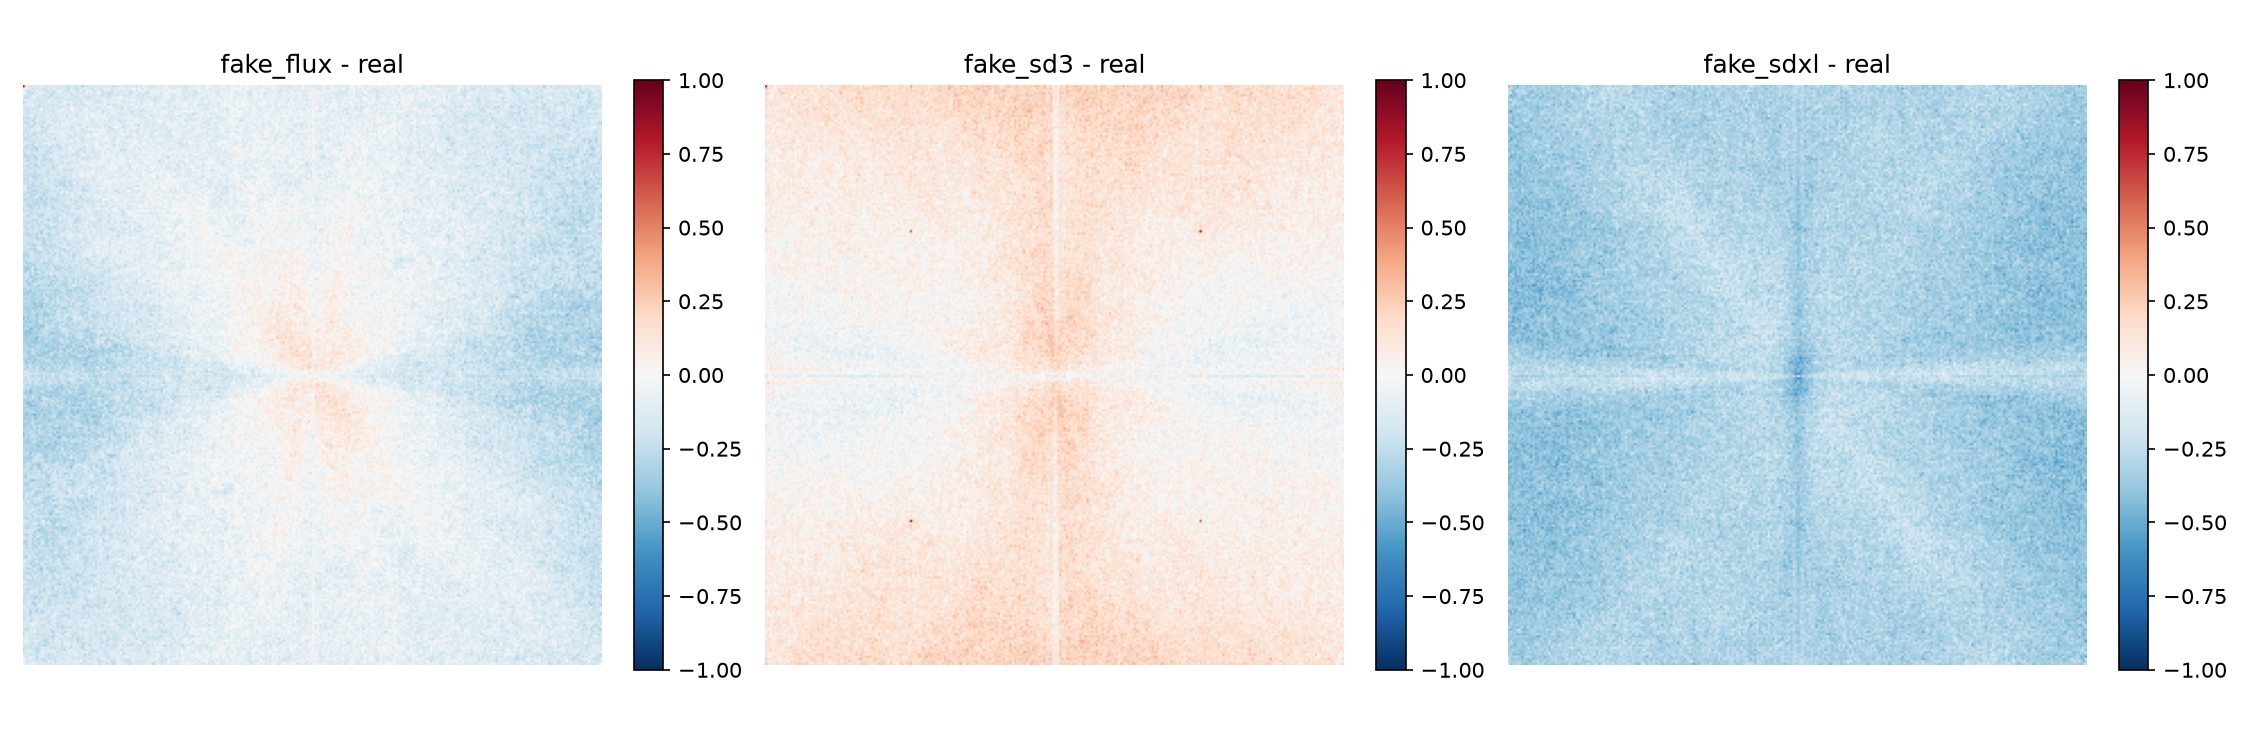
\includegraphics[width=\hsize]{figures/fig_spectra_diff.png}
\caption{Mean log-magnitude FFT difference from real images (fake minus
real), 300-image samples, for the three GenImage++ generators sharing one
real-image pool. Warm indicates more energy than real photographs at that
frequency, cool indicates less. SD3 is warm across most of the spectrum
while FLUX.1 and SDXL are mostly cool, matching the sign of the scalar
high-frequency measure in Table~\ref{tab:hfenergy}. BigGAN and GLIDE are
omitted because each is paired with its own real split rather than this
shared pool, so their maps are not on a comparable footing.}
\label{fig:spectradiff}
\end{figure}

We deliberately do not run a correlation between this scalar deviation and
fake-accuracy. With five generators, and a single summary statistic per
generator, any correlation coefficient would be computed on a handful of
points, where the estimate is dominated by which points happen to be
included and a $p$-value carries no useful information. We record the
spectral measurements as descriptive context and draw no inferential claim
from them. What we can say descriptively is that the ordering of generators
by spectral deviation does not match their ordering by detectability under
any detector in this study: BigGAN and GLIDE deviate from real-image
statistics by far the most (by $-283.5\%$ and $-234.3\%$) yet sit at
opposite ends of several detectors' accuracy rankings, while SD3's
uniquely positive deviation does not make it the outlier in any accuracy
column. Establishing whether spectral signature predicts detectability
would need a generator set large enough to support the test, which is a
different study from this one.

What holds up better as a descriptive pattern is architecture-family
clustering, though only for some of the detectors, and we report the
exceptions alongside the cases that fit. SD3 and FLUX.1, both Diffusion
Transformers built by different labs,
are each other's closest-scoring neighbour under UniversalFakeDetect (4.7
points apart within a 76-point spread) and under the GenImage++ CLIP
baseline (2.1 points within a 79-point spread), in each case the tightest
of the ten possible generator pairs. That happens despite SD3's spectral
deviation running opposite in sign to every other generator's, which is the
point: the two DiT generators behave alike for these detectors while
looking least alike in the frequency domain.

The pattern is not universal. For NPR the tightest pair is GLIDE/FLUX.1 and
SD3/FLUX.1 ranks fourth of ten, and for the GenImage++ ResNet-50 the
tightest pair is BigGAN/GLIDE with SD3/FLUX.1 third. CLIP-LoRA's entire
spread is 3.4 points, too compressed for any pairwise structure to mean
much. So architecture-family clustering describes two of five detectors
cleanly, and we present it as a pattern worth noting rather than a rule.
What is consistent across all of them is the negative claim: spectral
signature and detectability are separate axes, and neither should be
assumed to track the other.

\begin{table}[h]
\caption{High-frequency spectral energy, fake vs.\ real, per generator
(UniversalFakeDetect's native-resolution image pipeline; outer 20\% of
frequency radius, 300-image samples).}
\label{tab:hfenergy}
\begin{tabular*}{\hsize}{@{\extracolsep{\fill}}lrr@{}}
\toprule
Generator & Fake vs.\ real & Direction \\
\colrule
BigGAN & $-283.5\%$ & less high-freq \\
GLIDE & $-234.3\%$ & less high-freq \\
FLUX.1 & $-31.6\%$ & less high-freq \\
SD3 & $+15.1\%$ & \textbf{more} high-freq \\
SDXL & $-52.4\%$ & less high-freq \\
\botrule
\end{tabular*}
\end{table}

\subsection{Detectors fail by being confident, not uncertain}
\label{sec:confidence}

Figure~\ref{fig:scoredist} shows per-image predicted fake-probability
scores for UniversalFakeDetect across all five generators. On FLUX.1 and
SD3, the generators UniversalFakeDetect fails hardest on, the fake-image
score distribution does not sit near the 0.5 decision boundary; it
collapses almost entirely into the 0--0.1 bin, the same region occupied by
correctly classified real images. SDXL and GLIDE, the same detector's
better-handled modern/early-diffusion generators, retain a visible mass of
fake scores near 1.0. The failure mode this study documents is not
borderline uncertainty. It is confident misclassification: the detector
gives a low-uncertainty, wrong answer rather than an unsure one.

Reading that off a histogram is not enough to support the claim, so we
quantify it with expected calibration error (ECE), the standard
gap-between-confidence-and-correctness measure~\cite{guo2017calibration},
computed over 15 equal-width confidence bins. Table~\ref{tab:calibration}
gives ECE for every detector and generator. The numbers track the failure
pattern closely: UniversalFakeDetect's ECE is 0.042 on BigGAN, where it
works, and rises to 0.439 on FLUX.1, where it does not, meaning its average
confidence overstates its average correctness by more than 43 percentage
points. A detector that was merely uncertain on FLUX.1 would push its scores
toward 0.5 and produce a \emph{small} ECE alongside its low accuracy;
instead accuracy falls and calibration error rises together, which is the
signature of confident error rather than abstention. The same pattern holds
for the GenImage++ CLIP baseline on BigGAN (ECE 0.433 at 9.6\%
fake-accuracy), and most starkly for the GenImage++ ResNet-50 on BigGAN,
whose ECE of 0.503 accompanies a fake-accuracy of 0.4\%: it is wrong on
essentially every generated image and confident about it. The OMAT-hardened
CLIP-LoRA is the best-calibrated detector everywhere, never exceeding 0.020.

Across all 25 cells, calibration error and fake-accuracy move together
rather than independently, which is the point: these detectors do not
degrade gracefully into uncertainty as they leave their training
distribution, they stay confident and become wrong.

\begin{table}[h]
\caption{Expected calibration error (15 bins; lower is better) by detector
and generator. ECE rises with the failure severity in
Table~\ref{tab:results} rather than falling, which is the signature of
confident error rather than abstention.}
\label{tab:calibration}
\begin{tabular*}{\hsize}{@{\extracolsep{\fill}}lrrrrr@{}}
\toprule
Detector & BigGAN & GLIDE & FLUX.1 & SD3 & SDXL \\
\colrule
UniversalFakeDetect & 0.042 & 0.300 & 0.439 & 0.406 & 0.245 \\
NPR & 0.126 & 0.084 & 0.060 & 0.091 & 0.268 \\
GenImage++ ResNet-50 & 0.503 & 0.469 & 0.212 & 0.153 & 0.415 \\
GenImage++ CLIP & 0.433 & 0.120 & 0.034 & 0.031 & 0.076 \\
GenImage++ CLIP-LoRA & 0.015 & 0.015 & 0.020 & 0.015 & 0.012 \\
\botrule
\end{tabular*}
\end{table}

This matters for deployment. A detector that fails with high confidence
gives a downstream system no usable signal that it is operating outside its
competence: score thresholding, abstention, and human-review routing all
depend on low confidence tracking low reliability, and here it does the
opposite.

\begin{figure}[t]
\centering
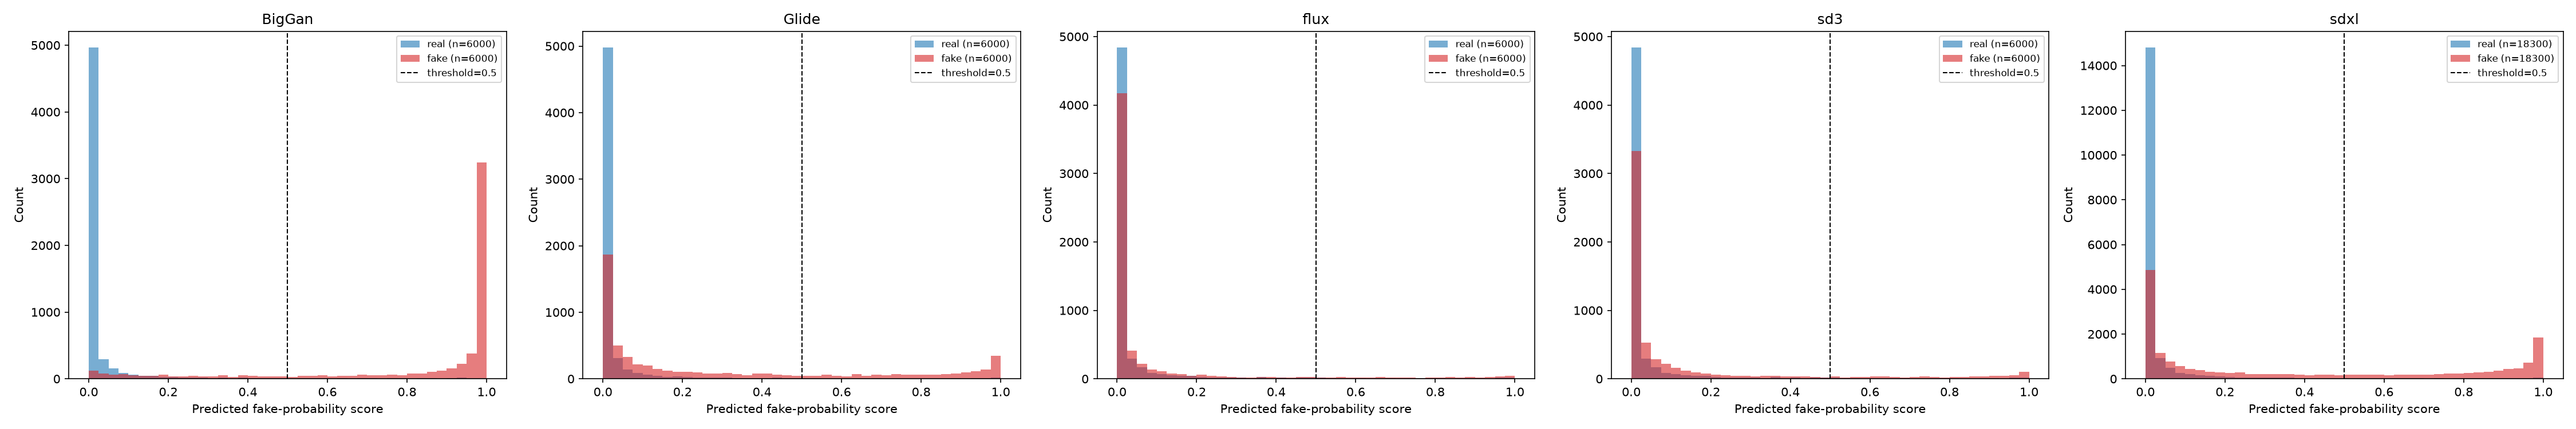
\includegraphics[width=\hsize]{figures/fig_score_dist_ufd.png}
\caption{UniversalFakeDetect predicted fake-probability scores, real
(blue) vs.\ fake (red), per generator. On FLUX.1/SD3 the fake distribution
collapses into the same low-score region as real images; on BigGAN the
pattern mirrors in the opposite direction.}
\label{fig:scoredist}
\end{figure}

Figure~\ref{fig:cmcontrast} makes the same point from a different angle,
contrasting two detectors on the identical 6{,}000 FLUX.1 fake images: NPR
correctly flags 5{,}864 of them, UniversalFakeDetect correctly flags 420.
Same images, same ground truth, opposite outcomes: this is the strongest
single illustration in this study that generalization failure is a
detector property, not a property of how hard a generator's outputs are to
detect in any absolute sense.

\begin{figure}[t]
\centering
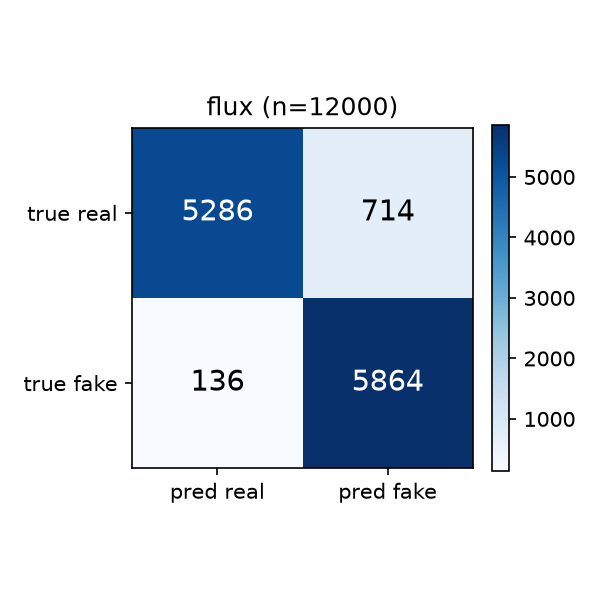
\includegraphics[width=0.48\hsize]{figures/fig_cm_npr_flux.png}\hfill
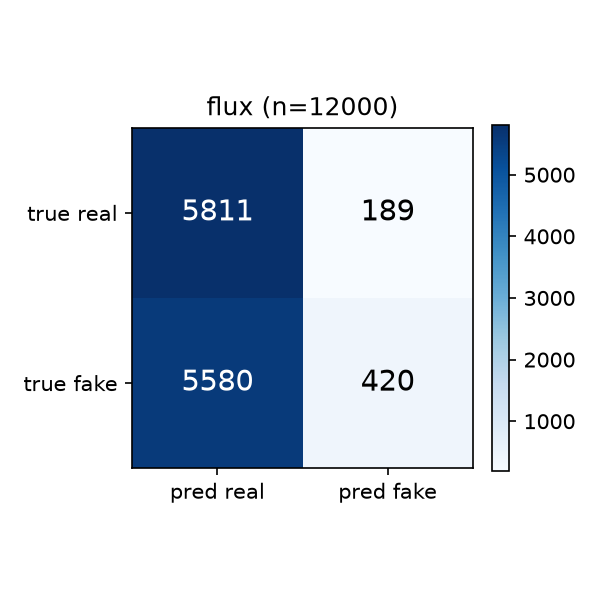
\includegraphics[width=0.48\hsize]{figures/fig_cm_ufd_flux.png}
\caption{Confusion matrices on the identical 12{,}000-image FLUX.1
evaluation set. Left: NPR. Right: UniversalFakeDetect. Same images, same
labels, opposite failure pattern.}
\label{fig:cmcontrast}
\end{figure}

\section{Discussion: a preprocessing-driven reproducibility hazard}
\label{sec:discussion}

While preparing Table~\ref{tab:results}, our measured fake-accuracy for
the GenImage++ CLIP baseline on BigGAN (9.6\%) sat roughly 6x below the
53.0\% overall accuracy we separately computed for the same run, and far
below the 62.66\% accuracy the source paper itself reports for its CLIP
baseline on GenImage's BigGAN subset. A 6x-scale disagreement between our
own measurement and a source paper's reported number, on what should be
the identical checkpoint and a same-named benchmark, is large enough that
it needed explaining before either number could be trusted, so we treat
the investigation itself as a contribution rather than a footnote.

We first ruled out an implementation bug in our own inference script by
reimplementing the source repository's actual released \texttt{kornia}-based
preprocessing function directly and running both versions, ours and
theirs, over the same sixteen images through the same loaded checkpoint.
The two implementations produced near-identical scores, ruling out a
preprocessing-implementation mismatch as the explanation and pointing the
investigation toward the data or the preprocessing \emph{choice} rather
than a coding error.

We then checked whether BigGAN's images themselves were the problem.
GenImage's BigGAN subset ships fakes at a native resolution of
128$\times$128 pixels, distinct from every other generator in the same
benchmark (GLIDE, for comparison, ships at 256$\times$256); this is
confirmed as the benchmark's own documented convention, not an artifact of
how we obtained the data. The officially released preprocessing function
resizes every input to 224$\times$224 regardless of its native size, which
means BigGAN's fakes are being force-upsampled by nearly a factor of two
before classification, while every other generator in the benchmark is
being downsampled or left closer to its target size. We tested whether
this specific resize direction was consequential by adding a second
preprocessing path that instead preserves native pixel scale, pasting the
image onto a black canvas at its original resolution rather than
interpolating it up to size. We re-ran the full 6{,}000-real/6{,}000-fake
BigGAN evaluation both ways for both the CLIP baseline and the OMAT
checkpoint (Figure~\ref{fig:biggancompare}, Table~\ref{tab:biggan}).

\begin{figure}[t]
\centering
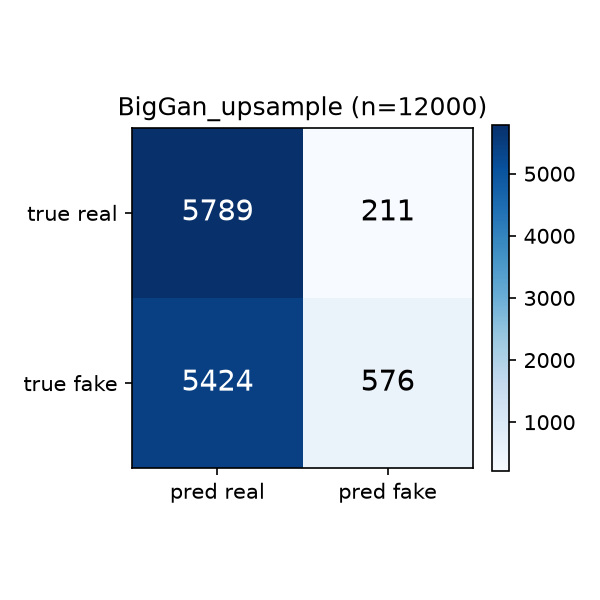
\includegraphics[width=0.48\hsize]{figures/fig_biggan_upsample.png}\hfill
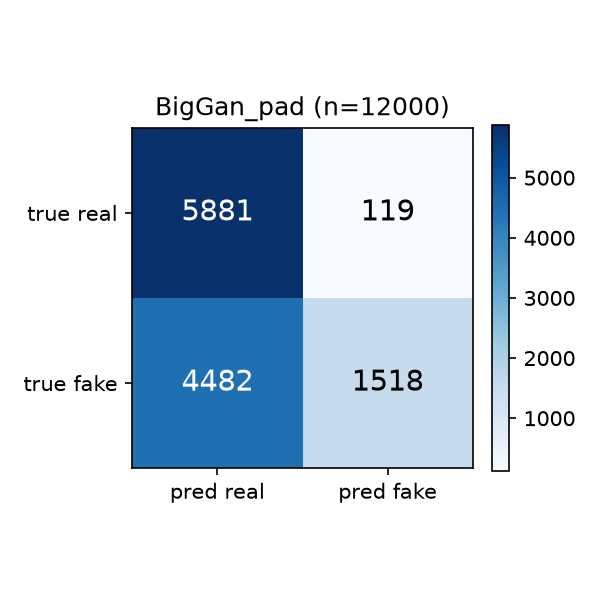
\includegraphics[width=0.48\hsize]{figures/fig_biggan_pad.png}
\caption{GenImage++ CLIP baseline on the full 12{,}000-image BigGAN
evaluation set. Left: official upsample-to-224 preprocessing. Right:
native-resolution-preserving padding. Same checkpoint, same images, same
threshold.}
\label{fig:biggancompare}
\end{figure}

\begin{table}[h]
\caption{BigGAN accuracy under two preprocessing choices, full 6{,}000/6{,}000
evaluation, both checkpoints.}
\label{tab:biggan}
\begin{tabular*}{\hsize}{@{\extracolsep{\fill}}p{2.6cm}p{2.1cm}rrrr@{}}
\toprule
Checkpoint & Preprocessing & Fake-acc & Overall acc & AP & AUC \\
\colrule
CLIP baseline & upsample (official) & 9.60 & 53.04 & 64.26 & 67.97 \\
CLIP baseline & padding (alternative) & 25.30 & \textbf{61.66} & 87.87 & 90.38 \\
CLIP-LoRA (OMAT) & upsample (official) & 99.70 & 97.26 & 99.55 & 99.70 \\
CLIP-LoRA (OMAT) & padding (alternative) & 16.28 & 54.70 & 64.78 & 69.13 \\
\botrule
\end{tabular*}
\end{table}

The padding variant moves the CLIP baseline's overall accuracy to 61.66\%,
within one point of the source paper's reported 62.66\%. Two effects
appear to compound to produce the original 6x gap: first, the source
paper's Table~1 accuracy column is almost certainly overall accuracy
(real and fake combined), while our first measurement was fake-only
accuracy, a metric-definition mismatch on our end, not a data problem;
second, the resize direction itself is a real effect we measured directly
rather than a mechanism we inferred. The same padding swap does the
opposite to the OMAT checkpoint, dropping it from 99.7\% to 16.3\%
fake-accuracy, which is consistent with the source paper's own
implementation notes stating that every fine-tuning strategy used a fixed
resize-to-224 pipeline during training. The OMAT model appears to have
learned to expect that specific pipeline, and native-padding pushes its
inputs out of that distribution in a way the never-fine-tuned baseline
does not suffer from.

We could not close the remaining small gap (61.66\% versus 62.66\%)
further: GenImage's official distribution is gated behind Baidu Yunpan
and Google Drive with no scriptable, authentication-free access, so we
could not pull a verified-authoritative image sample to test against
directly, and the source paper's own GenImage-benchmark evaluation script
is not among the code it released (the released code covers model
definition, checkpoint loading, and the adversarial-example generation
attack, not the cross-benchmark evaluation loop that produced Table~1).
We report this limit explicitly rather than assume the one-point residual
gap is fully explained.

\subsection{Does the effect generalize beyond BigGAN?}
\label{sec:glide-preproc}

A preprocessing effect demonstrated on one generator is an anecdote, so we
repeated the test on GLIDE, the only other generator in our set whose native
resolution is not 224$\times$224 (it ships at 256$\times$256).
Table~\ref{tab:glidepreproc} gives the result. For the CLIP baseline the
effect replicates in the same direction and at a smaller magnitude:
fake-accuracy rises from 69.1\% to 76.9\% and AUC from 94.0 to 97.4,
against a rise from 9.6\% to 25.3\% and AUC 68.0 to 90.4 on BigGAN. That
ordering is what the resolution gap predicts, since GLIDE needs only a mild
downsample to reach 224 while BigGAN is upsampled by nearly a factor of two.

For CLIP-LoRA the two generators behave completely differently. On GLIDE the
OMAT checkpoint is essentially unmoved (99.87\% to 99.77\% fake-accuracy);
on BigGAN it collapses (99.70\% to 16.28\%). Inspecting the two conditions
explains why, and qualifies the claim we made in
Section~\ref{sec:finding2}. Our native-resolution path center-crops images
larger than 224 and zero-pads images smaller than it. For GLIDE's
256$\times$256 inputs that is a pure center-crop with no border at all; for
BigGAN's 128$\times$128 inputs it produces a black frame covering 67.3\% of
the canvas. The two ``padding'' conditions are therefore not the same
operation, and the BigGAN collapse is confounded between two candidate
causes: the absence of smooth interpolation, and the presence of a large
out-of-distribution black border.

\begin{table}[h]
\caption{Padding versus official upsampling on the two generators whose
native resolution is not 224$\times$224. Full evaluation sets. The GLIDE
``padding'' condition is a pure center-crop; the BigGAN one introduces a
black border over 67.3\% of the canvas, which is why the two are not
directly comparable.}
\label{tab:glidepreproc}
\begin{tabular*}{\hsize}{@{\extracolsep{\fill}}llrrr@{}}
\toprule
Generator & Checkpoint / preprocessing & Fake & Real & AUC \\
\colrule
BigGAN (128) & CLIP, upsample & 9.60 & 96.48 & 67.97 \\
BigGAN (128) & CLIP, padding & 25.30 & 98.02 & 90.38 \\
BigGAN (128) & CLIP-LoRA, upsample & 99.70 & 94.82 & 99.70 \\
BigGAN (128) & CLIP-LoRA, padding & 16.28 & 93.12 & 69.13 \\
GLIDE (256) & CLIP, upsample & 69.13 & 96.05 & 94.03 \\
GLIDE (256) & CLIP, padding & 76.93 & 98.20 & 97.44 \\
GLIDE (256) & CLIP-LoRA, upsample & 99.87 & 94.87 & 99.82 \\
GLIDE (256) & CLIP-LoRA, padding & 99.77 & 92.82 & 99.88 \\
\botrule
\end{tabular*}
\end{table}

We therefore ran a third condition on BigGAN that separates the two: a
nearest-neighbour upsample to 224$\times$224, which removes smooth
interpolation exactly as padding does but introduces no border.

\subsection{Separating interpolation from border artifacts}
\label{sec:disentangle}

Table~\ref{tab:disentangle} reports all three conditions on matched samples
of 2{,}000 images per class. The two candidate causes turn out to be
separable, and they act through different mechanisms.

\begin{table}[h]
\caption{BigGAN, CLIP-LoRA (OMAT), three preprocessing conditions on
matched 2{,}000-image-per-class samples. Removing interpolation costs
accuracy but preserves ranking (AUC 97.90); adding a zero-padding border
destroys the ranking as well (AUC 60.36). The final row gives the
non-adversarial CLIP baseline under the same nearest-neighbour condition.}
\label{tab:disentangle}
\begin{tabular*}{\hsize}{@{\extracolsep{\fill}}lrrr@{}}
\toprule
Condition & Fake & Real & AUC \\
\colrule
CLIP-LoRA, upsample (interpolation, no border) & 99.25 & 95.50 & 99.63 \\
CLIP-LoRA, nearest (no interpolation, no border) & 61.45 & 99.35 & 97.90 \\
CLIP-LoRA, padding (no interpolation, 67\% border) & 5.30 & 93.45 & 60.36 \\
CLIP baseline, nearest (no interpolation, no border) & 11.05 & 100.00 & 90.72 \\
\botrule
\end{tabular*}
\end{table}

Dropping smooth interpolation alone costs CLIP-LoRA 37.8 points of
fake-accuracy (99.25\% to 61.45\%) while its AUC falls only 1.7 points, from
99.63 to 97.90. An accuracy collapse with the ranking left intact is a
threshold problem: the model still orders generated above real almost as
well as before, but the score distribution has shifted out from under the
fixed 0.5 cut. Adding the zero-padding border on top of that is a different
kind of damage. Fake-accuracy falls to 5.30\% and AUC to 60.36, close
enough to chance that no threshold would recover it, so the border removes
discriminative information rather than merely relocating it.

This corrects the reading we gave in Section~\ref{sec:finding2}. The
dramatic BigGAN collapse of the OMAT checkpoint is driven mainly by the
large out-of-distribution border our native-resolution path introduces for
128$\times$128 inputs, not by the absence of interpolation. The accurate
statement is narrower and more useful: OMAT's hardening survives a change
of interpolation kernel in ranking terms while losing threshold
calibration, and fails outright only when the input is distorted in a way
that has no counterpart in its training pipeline. It also explains the
GLIDE result, where the native-resolution path introduces no border at all
and the OMAT checkpoint is accordingly untouched.

The CLIP baseline behaves in the opposite direction on the same axis. Under
nearest-neighbour upsampling its AUC rises to 90.72 from the 67.97 it
records under the official bicubic pipeline, so for a detector never
fine-tuned against a fixed input pipeline, the smooth interpolation applied
to a 128$\times$128 generator output is itself destroying usable signal.
Two checkpoints trained on identical data thus prefer opposite
preprocessing, which is the sharpest form of the reproducibility point this
section makes: there is no single preprocessing choice that is neutral
across detectors, so a benchmark that fixes one is implicitly favouring
some detectors over others.

Taken together, the three experiments in this section support one claim:
the same checkpoint, on the same images, at the same threshold, produces
materially different published-style accuracy numbers under defensible
preprocessing conventions, and the direction of the change is not
consistent even across checkpoints trained on identical data. A resize
decision that no reader would expect to matter for a frozen-backbone
classifier moved one checkpoint's reported accuracy by more than 15
percentage points. Because preprocessing pipelines are often
under-specified in released detector code, and because cross-generator
accuracy tables are routinely compared across papers that each apply their
own convention, this is not a caution specific to our pipeline. A reader
comparing published accuracy numbers across papers should treat a
resize or crop mismatch as a plausible, checkable explanation for an
unexplained gap before concluding that either number is wrong.

The access barrier we hit while chasing the residual one-point gap suggests
a concrete recommendation for benchmark authors, which we state separately
because it applies well beyond this one dataset.
A benchmark intended for cross-paper accuracy comparison should ship a
small, scriptable, authentication-free verification subset: a few hundred
images with published per-image checksums, retrievable without a login,
together with the exact preprocessing function and metric definition used
to produce the headline table. None of that requires redistributing the
full dataset or solving the hosting problem that pushes large benchmarks
onto gated storage in the first place. Had such a subset existed for
GenImage, the investigation in this section would have taken an afternoon
instead of several days, and the residual one-point gap would be resolved
rather than merely bounded. The cost to a benchmark author is a few
megabytes; the cost of its absence is that every downstream paper's numbers
become difficult to compare against every other's.

\section{JPEG re-encoding robustness, and a dataset bias it exposes}
\label{sec:robustness}

Images that reach a real detector have usually been re-encoded at least
once by whatever platform carried them. We therefore re-ran the FLUX.1
evaluation with every image re-encoded at JPEG quality 75 before
classification, holding the image sample fixed at 2{,}000 per class so the
clean and compressed conditions are paired. Table~\ref{tab:jpeg} reports
both.

\begin{table}[h]
\caption{FLUX.1 evaluation before and after JPEG quality-75 re-encoding
(2{,}000 images per class, same sample in both conditions). NPR loses all
discriminative signal, its AUC falling to chance; the CLIP-family detectors
lose accuracy but largely retain ranking ability.}
\label{tab:jpeg}
\begin{tabular*}{\hsize}{@{\extracolsep{\fill}}lcccc@{}}
\toprule
& \multicolumn{2}{c}{Fake-acc (\%)} & \multicolumn{2}{c}{AUC} \\
Detector & clean & JPEG-75 & clean & JPEG-75 \\
\colrule
UniversalFakeDetect & 7.30 & 6.00 & 61.19 & 55.54 \\
NPR & 98.00 & \textbf{1.50} & 97.10 & \textbf{50.63} \\
GenImage++ ResNet-50 & 69.45 & 58.00 & 91.27 & 88.48 \\
GenImage++ CLIP & 89.60 & 59.80 & 98.56 & 97.28 \\
GenImage++ CLIP-LoRA & 97.65 & 41.90 & 99.30 & 90.67 \\
\botrule
\end{tabular*}
\end{table}

The headline number is NPR. It is the strongest detector on FLUX.1 by a
wide margin in the clean condition (98.0\% fake-accuracy) and it is
destroyed by ordinary compression, falling to 1.50\% with an AUC of 50.63,
which is chance. This is mechanistically unsurprising once stated: NPR
detects generated images from up-sampling artifacts in neighbouring-pixel
relationships, and JPEG quantisation attacks exactly the high-frequency
content those artifacts live in. The practical implication is sharp. The
detector a deployer would pick from a clean-data leaderboard is the one
that fails most completely on data that has passed through any normal
image pipeline.

The CLIP-family detectors degrade differently and more gracefully. The
GenImage++ CLIP baseline loses 29.8 points of fake-accuracy but only 1.3
points of AUC (98.56 to 97.28), and CLIP-LoRA loses 55.8 points of accuracy
against 8.6 of AUC. An accuracy drop far larger than the AUC drop means the
score \emph{ranking} still separates real from generated while the fixed
0.5 threshold no longer sits in the right place. That failure is
recoverable by recalibrating a threshold; NPR's is not, because at an AUC
of 50.6 there is no threshold that would help.

\subsection{A compression confound in the underlying benchmarks}
\label{sec:jpeg-confound}

This experiment also surfaced something about the datasets that qualifies
our own absolute numbers, and we report it prominently rather than in a
footnote. Across all five generators in this study, every generated image
is distributed as PNG while every real image is distributed as JPEG: BigGAN
and GLIDE fakes are PNG at 128$\times$128 and 256$\times$256, GenImage++
fakes are PNG at 1024$\times$1024, and all real images are ImageNet JPEGs.
Real and generated images therefore differ systematically in compression
history, not only in whether a generator produced them, and a detector
sensitive to compression artifacts can score well by exploiting that
difference instead of any generative fingerprint.

The bias is documented for GenImage by Grommelt et
al.~\cite{grommelt2024jpeg}, who report that removing JPEG and
image-dimension confounds changes cross-generator detector performance by
more than 11 percentage points. Our JPEG experiment supplies a direct
estimate of its size for the most artifact-sensitive detector we test: once
the generated images carry JPEG compression too, NPR's ability to separate
the classes vanishes entirely. We cannot conclude from one experiment that
NPR's clean 98.0\% on FLUX.1 is \emph{entirely} a compression artifact,
because JPEG re-encoding also destroys genuine generative traces, and those
two explanations predict the same collapse. What we can say is that NPR's
clean FLUX.1 result should not be read as a pure measurement of generative
artifact detection, and that any detector's absolute accuracy on these
benchmarks carries this confound.

Two things limit the damage to this paper's claims. All five detectors were
evaluated on exactly the same images, so the cross-detector comparisons in
Section~\ref{sec:results}, including every paired test in
Section~\ref{sec:significance}, remain valid as comparisons even if the
absolute levels are inflated by a shared bias. And the confound is a
property of the real/fake pairing, so it cannot explain the
Section~\ref{sec:finding-shape} result, where two detectors on identical
images produce identical difficulty \emph{orderings} at very different
accuracy levels. A version of this study on a compression-balanced
benchmark, such as the debiased GenImage variant released with
\cite{grommelt2024jpeg}, is the obvious next step and we flag it as the
most important single follow-up.

\section{Limitations}
\label{sec:limitations}

Detector diversity in this study is narrower than ``five detectors''
suggests: three of the five (UniversalFakeDetect, the GenImage++ CLIP
baseline, and its LoRA variant) are CLIP-embedding classifiers sharing the
same backbone family. The two convolutional detectors, NPR and the
GenImage++ ResNet-50, are structurally distinct from that family and from
each other in training data, which is why we lean on them when separating
architecture effects from training-distribution effects. Findings that
hold across all five detectors are on firmer ground than findings drawn
from the CLIP-family detectors alone, and we have tried to mark which is
which throughout. A genuinely independent detector family, for instance a
diffusion-reconstruction method such as DIRE~\cite{wang2023dire}, would
strengthen the design further and is the most valuable single addition
future work could make.

Real-image overlap between the ImageNet images used to train the
GenImage++ checkpoints' SDv1.4 subset and the ImageNet-derived real-image
pools used in our own evaluation is an open question we could not resolve
from released materials. This would not explain the fake-accuracy findings
that anchor this paper's main claims, since it concerns only the real-image
side of the evaluation, but it could inflate real-accuracy or AP figures
for the GenImage++ checkpoints slightly, and we flag it as unconfirmed
rather than assert either outcome.

The exact training composition of the two GenImage++ checkpoints beyond
what is stated in the source paper's own text was not independently
re-verified against internal training logs we do not have access to; our
leakage conclusion (Section~\ref{sec:methods-leakage}) rests on the source
paper's own reported methodology being accurate.

GenImage++'s own generator outputs, while confirmed test-only by the
dataset's documentation, were generated and released by a third party; we
did not independently verify their generation prompts or pipeline beyond
what the dataset's own card states.

Cross-detector real-accuracy on FLUX.1, SD3, and SDXL is an unpaired
comparison. Because GenImage++ ships no real images, each detector's run
drew its own random sample from the shared 162{,}000-image ImageNet pool,
and the resulting real-image sets overlap only incidentally across
detectors (7 of 6{,}000 images for FLUX.1 and SD3, 200 of 18{,}300 for
SDXL). The fake-image sets are identical across all five detectors for
every generator, so the fake-accuracy comparisons and every paired test in
Section~\ref{sec:significance} are properly paired; the real-accuracy
column for those three generators compares equal-sized independent draws
from one pool rather than matched images. BigGAN and GLIDE use each
generator's own paired real split and are fully matched on both classes.

All detectors are evaluated at their native output resolution handling and
at a fixed decision threshold of 0.5 (Section~\ref{sec:methods-protocol}).
We do not tune per-detector thresholds, so the accuracy figures should be
read as out-of-the-box behavior rather than as each detector's best
achievable operating point; AUC and AP, which are threshold-free, are
reported alongside for exactly this reason.

Finally, a note on cost, since we motivate this study partly by deployment
concerns. Measured on the single 8~GB consumer GPU used throughout, the
three CLIP ViT-L/14 detectors run at 7.4--7.6 images per second
(132--139~ms per image), while NPR's ResNet-50 over pixel-artifact features
runs at 229--320 images per second (3.1--4.4~ms per image), roughly 35 times
faster. That gap is not incidental to the paper's argument. NPR is both the
cheapest detector here and the strongest on the two Diffusion Transformer
generators, so the detector a deployer would pick on throughput grounds is
not the one they would pick from published headline accuracy, and the
combination we recommend in Section~\ref{sec:conclusion} (pairing detectors
with different training lineages) is cheaper than it might appear. We report
throughput rather than isolated forward-pass latency because batch
inference is the realistic deployment mode, and we make no claim about
optimised or quantised implementations of any of these models.

\section{Conclusion}
\label{sec:conclusion}

Five pretrained AI-generated image detectors, evaluated against five
generators spanning three architecture families with training/test leakage
verified absent, disagree about which generator is hardest, and the
disagreement is statistically real rather than sampling noise. What
predicts a detector's weak spot is its training distribution, not how
recent the generator is: the oldest generator in our set, BigGAN, is the
single hardest case for two detectors and among the easiest for two
others.

Adding a detector trained on the same data as an existing one but built on
a different architecture sharpens that claim into something more useful
than ``training data matters.'' Those two detectors rank the five
generators in exactly the same order while differing by 37.6 points in
mean accuracy. On the evidence available here, the training distribution
appears to fix the shape of a detector's failure profile and the
representation to fix its level, which would mean that swapping in a
stronger backbone raises a detector's accuracy without moving its blind
spot. That is a two-detector observation and we mark it as such, but it is
a testable one, and it predicts that ensembling detectors chosen for
different \emph{training lineages} should beat ensembling detectors chosen
for different architectures.

The failure mode itself is what makes these gaps consequential. Calibration
error rises alongside error rate rather than falling, so a detector leaving
its training distribution does not signal its own unreliability through
lower confidence; it stays confident and becomes wrong. Adversarial
training on on-manifold latent perturbations both closes most of the
accuracy gap and produces by far the best-calibrated detector we test,
which is the most encouraging result in the study. Its robustness proved
more durable than our first reading suggested: it survives a change of
interpolation kernel with its ranking nearly intact and fails only under an
input distortion with no counterpart in its training pipeline.

Two findings should temper how any of these accuracy numbers are used.
Ordinary JPEG re-encoding, the kind any image undergoes when it passes
through a platform, takes NPR from the best FLUX.1 detector we measure
(98.0\%) to chance-level AUC, so the detector a clean-data leaderboard
would recommend is the one least suited to deployment. And in every
benchmark we use, generated images are distributed as PNG while real images
are JPEG, a compression asymmetry documented by prior
work~\cite{grommelt2024jpeg} that our own experiment shows can account for
a large share of one detector's apparent skill. Cross-detector comparisons
survive this, since every detector saw the same images, but absolute
accuracies on these benchmarks should be treated as upper bounds.

Finally, the investigation that produced that last caveat began as an
unexplained 6x gap against a published number and ended in a
metric-definition mismatch plus a real preprocessing effect that we
replicate on a second generator. We report it at length because the hazard
is not ours alone: a resize convention that no reader would expect to
matter changes published-style accuracy by more than 15 points, in
opposite directions for two checkpoints trained on identical data. Until
benchmarks ship the small, scriptable verification subsets we recommend in
Section~\ref{sec:discussion}, cross-paper accuracy comparisons in this
literature should be read with that possibility in mind. Every result here
was produced by inference over existing checkpoints and released datasets,
with no training and no image generation, on a single consumer GPU.

\section{Ethical and dual-use considerations}
\label{sec:ethics}

Work that documents where AI-generated image detectors fail is dual-use by
construction: the same table that tells a platform which detector to avoid
deploying against Diffusion Transformer imagery also tells someone trying to
evade detection which generator to prefer. We think publication is still the
right call here, for three reasons. The detectors and generators we study are
already public, so the failure modes are discoverable by anyone willing to run
the same inference we ran; nothing in this paper is a capability that did not
previously exist. The information asymmetry currently runs against defenders,
who often deploy a single detector on the implicit assumption that a published
accuracy number transfers, which our results show it does not. And the
concrete recommendations that follow from our findings, namely combining
detectors with different training lineages and reporting calibration and
preprocessing alongside accuracy, are defensive rather than evasive: an
adversary gains little from them, while a deployer gains a great deal.

Two narrower cautions apply. First, none of the detectors evaluated here
should be used as sole evidence in any consequential decision about a
person, given that the best-calibrated detector in our study still
misclassifies a meaningful fraction of real images and the worst is
confidently wrong most of the time on some generators. Second, our results
are measured on ImageNet-derived object and scene imagery; we make no claim
about detector behavior on images of people, and the face-manipulation
setting discussed in Section~\ref{sec:related} is out of scope entirely.

\section*{Acknowledgements}

\appendix
\section{Data and code availability}
Detector checkpoints and evaluation datasets used in this study are the
original authors' public releases, cited in Table~\ref{tab:detectors} and
Section~\ref{sec:methods}. The evaluation harness, the per-image prediction
scores for every detector and generator reported here, the paired
significance tests, the calibration computations, and the
preprocessing-sensitivity analysis of Section~\ref{sec:discussion} will be
released publicly upon publication; the repository link is withheld here
only to preserve review anonymity and will be inserted in the
camera-ready version.

\begin{thebibliography}{99}

\bibitem{wang2020cnndetect}
Wang, Sheng-Yu, Oliver Wang, Richard Zhang, Andrew Owens, and Alexei A.\ Efros.
(2020) ``CNN-generated images are surprisingly easy to spot... for now.''
\textit{Proceedings of the IEEE/CVF Conference on Computer Vision and
Pattern Recognition}: 8695--8704.

\bibitem{genimage2023}
Zhu, Mingjian, Hanting Chen, Qiangyu Yan, Xudong Huang, Guanyu Lin, Wei Li,
Zhijun Tu, Hailin Hu, Jie Hu, and Yunhe Wang. (2023) ``GenImage: A
million-scale benchmark for detecting AI-generated image.''
\textit{Advances in Neural Information Processing Systems} \textbf{36}:
77771--77782.

\bibitem{ojha2023universal}
Ojha, Utkarsh, Yuheng Li, and Yong Jae Lee. (2023) ``Towards Universal Fake
Image Detectors that Generalize Across Generative Models.''
\textit{Proceedings of the IEEE/CVF Conference on Computer Vision and
Pattern Recognition}: 24480--24489.

\bibitem{tan2024npr}
Tan, Chuangchuang, Yao Zhao, Shikui Wei, Guanghua Gu, Ping Liu, and Yunchao
Wei. (2024) ``Rethinking the Up-Sampling Operations in CNN-based
Generative Network for Generalizable Deepfake Detection.''
\textit{Proceedings of the IEEE/CVF Conference on Computer Vision and
Pattern Recognition}: 28130--28139.

\bibitem{zhou2025omat}
Zhou, Yue, Xinan He, KaiQing Lin, Bin Fan, Feng Ding, and Bin Li. (2025)
``Breaking Latent Prior Bias in Detectors for Generalizable AIGC Image
Detection.'' \textit{arXiv preprint arXiv:2506.00874}.

\bibitem{flux2024}
Black Forest Labs. (2024) ``FLUX.'' \url{https://github.com/black-forest-labs/flux}.

\bibitem{esser2024sd3}
Esser, Patrick, Sumith Kulal, Andreas Blattmann, Rahim Entezari, Jonas
M\"{u}ller, Harry Saini, Yam Levi, Dominik Lorenz, Axel Sauer, Frederic
Boesel, et al. (2024) ``Scaling rectified flow transformers for
high-resolution image synthesis.'' \textit{Forty-first International
Conference on Machine Learning}.

\bibitem{brock2019biggan}
Brock, Andrew, Jeff Donahue, and Karen Simonyan. (2019) ``Large scale GAN
training for high fidelity natural image synthesis.'' \textit{International
Conference on Learning Representations}.

\bibitem{nichol2021glide}
Nichol, Alex, Prafulla Dhariwal, Aditya Ramesh, Pranav Shyam, Pamela
Mishkin, Bob McGrew, Ilya Sutskever, and Mark Chen. (2021) ``GLIDE:
Towards photorealistic image generation and editing with text-guided
diffusion models.'' \textit{arXiv preprint arXiv:2112.10741}.

\bibitem{podell2023sdxl}
Podell, Dustin, Zion English, Kyle Lacey, Andreas Blattmann, Tim Dockhorn,
Jonas M\"{u}ller, Joe Penna, and Robin Rombach. (2023) ``SDXL: Improving
latent diffusion models for high-resolution image synthesis.''
\textit{arXiv preprint arXiv:2307.01952}.

\bibitem{radford2021clip}
Radford, Alec, Jong Wook Kim, Chris Hallacy, Aditya Ramesh, Gabriel Goh,
Sandhini Agarwal, Girish Sastry, Amanda Askell, Pamela Mishkin, Jack Clark,
et al.\ (2021) ``Learning transferable visual models from natural language
supervision.'' \textit{International Conference on Machine Learning}:
8748--8763.

\bibitem{hu2022lora}
Hu, Edward J., Yelong Shen, Phillip Wallis, Zeyuan Allen-Zhu, Yuanzhi Li,
Shean Wang, Lu Wang, and Weizhu Chen. (2022) ``LoRA: Low-rank adaptation of
large language models.'' \textit{International Conference on Learning
Representations}.

\bibitem{rombach2022ldm}
Rombach, Robin, Andreas Blattmann, Dominik Lorenz, Patrick Esser, and
Bj\"{o}rn Ommer. (2022) ``High-resolution image synthesis with latent
diffusion models.'' \textit{Proceedings of the IEEE/CVF Conference on
Computer Vision and Pattern Recognition}: 10684--10695.

\bibitem{peebles2023dit}
Peebles, William, and Saining Xie. (2023) ``Scalable diffusion models with
transformers.'' \textit{Proceedings of the IEEE/CVF International
Conference on Computer Vision}: 4195--4205.

\bibitem{goodfellow2014gan}
Goodfellow, Ian, Jean Pouget-Abadie, Mehdi Mirza, Bing Xu, David
Warde-Farley, Sherjil Ozair, Aaron Courville, and Yoshua Bengio. (2020)
``Generative adversarial networks.'' \textit{Communications of the ACM}
\textbf{63} (11): 139--144.

\bibitem{xu2025seeds}
Xu, Katherine, Lingzhi Zhang, and Jianbo Shi. (2025) ``Good seed makes
good crop: Discovering secret seeds in text-to-image diffusion models.''
\textit{IEEE/CVF Winter Conference on Applications of Computer Vision}:
3024--3034.

\bibitem{wang2023dire}
Wang, Zhendong, Jianmin Bao, Wengang Zhou, Weilun Wang, Hezhen Hu, Hong
Chen, and Houqiang Li. (2023) ``DIRE for diffusion-generated image
detection.'' \textit{Proceedings of the IEEE/CVF International Conference
on Computer Vision}: 22445--22455.

\bibitem{yan2024chameleon}
Yan, Shilin, Ouxiang Li, Jiayin Cai, Yanbin Hao, Xiaolong Jiang, Yao Hu,
and Weidi Xie. (2024) ``A sanity check for AI-generated image detection.''
\textit{arXiv preprint arXiv:2406.19435}.

\bibitem{qian2020freq}
Qian, Yuyang, Guojun Yin, Lu Sheng, Zixuan Chen, and Jing Shao. (2020)
``Thinking in frequency: Face forgery detection by mining
frequency-aware clues.'' \textit{European Conference on Computer Vision}:
86--103.

\bibitem{tan2025c2pclip}
Tan, Chuangchuang, Renshuai Tao, Huan Liu, Guanghua Gu, Baoyuan Wu, Yao
Zhao, and Yunchao Wei. (2025) ``C2P-CLIP: Injecting category common
prompt in CLIP to enhance generalization in deepfake detection.''
\textit{Proceedings of the AAAI Conference on Artificial Intelligence}
\textbf{39}: 7184--7192.

\bibitem{rossler2019ff}
R\"{o}ssler, Andreas, Davide Cozzolino, Luisa Verdoliva, Christian Riess,
Justus Thies, and Matthias Nie{\ss}ner. (2019) ``FaceForensics++: Learning
to detect manipulated facial images.'' \textit{Proceedings of the IEEE/CVF
International Conference on Computer Vision}: 1--11.

\bibitem{li2020celebdf}
Li, Yuezun, Xin Yang, Pu Sun, Honggang Qi, and Siwei Lyu. (2020)
``Celeb-DF: A large-scale challenging dataset for deepfake forensics.''
\textit{Proceedings of the IEEE/CVF Conference on Computer Vision and
Pattern Recognition}: 3207--3216.

\bibitem{chollet2017xception}
Chollet, Fran\c{c}ois. (2017) ``Xception: Deep learning with depthwise
separable convolutions.'' \textit{Proceedings of the IEEE Conference on
Computer Vision and Pattern Recognition}: 1251--1258.

\bibitem{frank2020leveraging}
Frank, Joel, Thorsten Eisenhofer, Lea Sch\"{o}nherr, Asja Fischer, Dorothea
Kolossa, and Thorsten Holz. (2020) ``Leveraging frequency analysis for deep
fake image recognition.'' \textit{International Conference on Machine
Learning}: 3247--3258.

\bibitem{selvaraju2017gradcam}
Selvaraju, Ramprasaath R., Michael Cogswell, Abhishek Das, Ramakrishna
Vedantam, Devi Parikh, and Dhruv Batra. (2017) ``Grad-CAM: Visual
explanations from deep networks via gradient-based localization.''
\textit{Proceedings of the IEEE International Conference on Computer
Vision}: 618--626.

\bibitem{guo2017calibration}
Guo, Chuan, Geoff Pleiss, Yu Sun, and Kilian Q. Weinberger. (2017) ``On
calibration of modern neural networks.'' \textit{International Conference
on Machine Learning}: 1321--1330.

\bibitem{mcnemar1947}
McNemar, Quinn. (1947) ``Note on the sampling error of the difference
between correlated proportions or percentages.'' \textit{Psychometrika}
\textbf{12} (2): 153--157.

\bibitem{grommelt2024jpeg}
Grommelt, Patrick, Louis Weiss, Franz-Josef Pfreundt, and Janis Keuper.
(2024) ``Fake or JPEG? Revealing common biases in generated image detection
datasets.'' \textit{arXiv preprint arXiv:2403.17608}.

\end{thebibliography}

\end{document}
